\subsection{Validation and Testing Procedures for Model Evaluation}\label{subsec:validation_testing_procedures}
This section describes the validation and testing procedures our experiments follow.
Selecting appropriate testing procedures is crucial for ensuring the validity and reliability of the results.
For that reason, we delineate a methodological approach that ensures our models are accurate and generalizable.

We have chosen to test and evaluate all our experiments using both cross-validation and a separate test set.
Evaluating results solely on the test set could lead to models that are overly specialized to the test set.
This occurs when searching for the optimal configuration of hyperparameters specifically tailored to the test set.
However, our objective is to develop models that demonstrate high accuracy and robustness, even on entirely unseen data.
To achieve this, we employ k-fold cross-validation to ensure our models have high generalizability, thereby increasing the likelihood that they will perform as expected on new data.

We use an $80\%/20\%$ split for training and testing sets. The training set is further subdivided into $k$ folds, which are used for cross validation.

While we employ conventional techniques like holdout sets and k-fold cross validation, \gls{libs} data imposes additional challenges to the process.

One of the primary challenges is preventing data leakage.
As per concentration matrix $\mathbf{C}$ in Section~\ref{sec:problem_definition}, each target only has one ground truth concentration value per oxide.
However, each target is shot at multiple locations, resulting in multiple instances of the same target in the dataset, as shown in Table~\ref{tab:final_dataset_example}.
Although the intensity values vary for each location, they fundamentally represent measurements of the same target.
If we were to randomly split the dataset, some locations from a target could end up in the testing set while others remain in the training set.
This would cause data leakage, as the testing set would no longer consist solely of unseen targets.
To prevent this, we ensure that each target is represented only once in the dataset by grouping data from all locations on a given target.

Furthermore, the limited availability of data, as mentioned in Section~\ref{sec:problem_definition}, poses another significant challenge due to the difficult collection process.
The dataset we use consists of 408 samples, which is relatively large by \gls{libs} standards.
However, there are only a few samples with concentration values for the oxides in the targets that are either very high or very low compared to the rest of the data.
These less frequent high and low concentration values can be problematic.
If such values end up in the test set, the model may be evaluated on data points outside the range it was trained on.
This situation can lead to an inaccurate assessment of the model's performance, as it might not handle these less common concentration ranges effectively.

When performing a random split of the dataset into multiple folds for cross-validation, as well as for training and testing sets, this small number of extreme values can result in an uneven distribution.
The presence or absence of these extreme values in any given fold can heavily influence the model's performance metrics.
If extreme values are disproportionately allocated to either the training or testing sets, the resulting model may struggle to generalize accurately.
This uneven distribution can lead to models that perform well on the majority of the data but fail to predict accurately for these extreme concentration values, which are critical in many practical applications.

\begin{figure*}[h!]
    \centering
    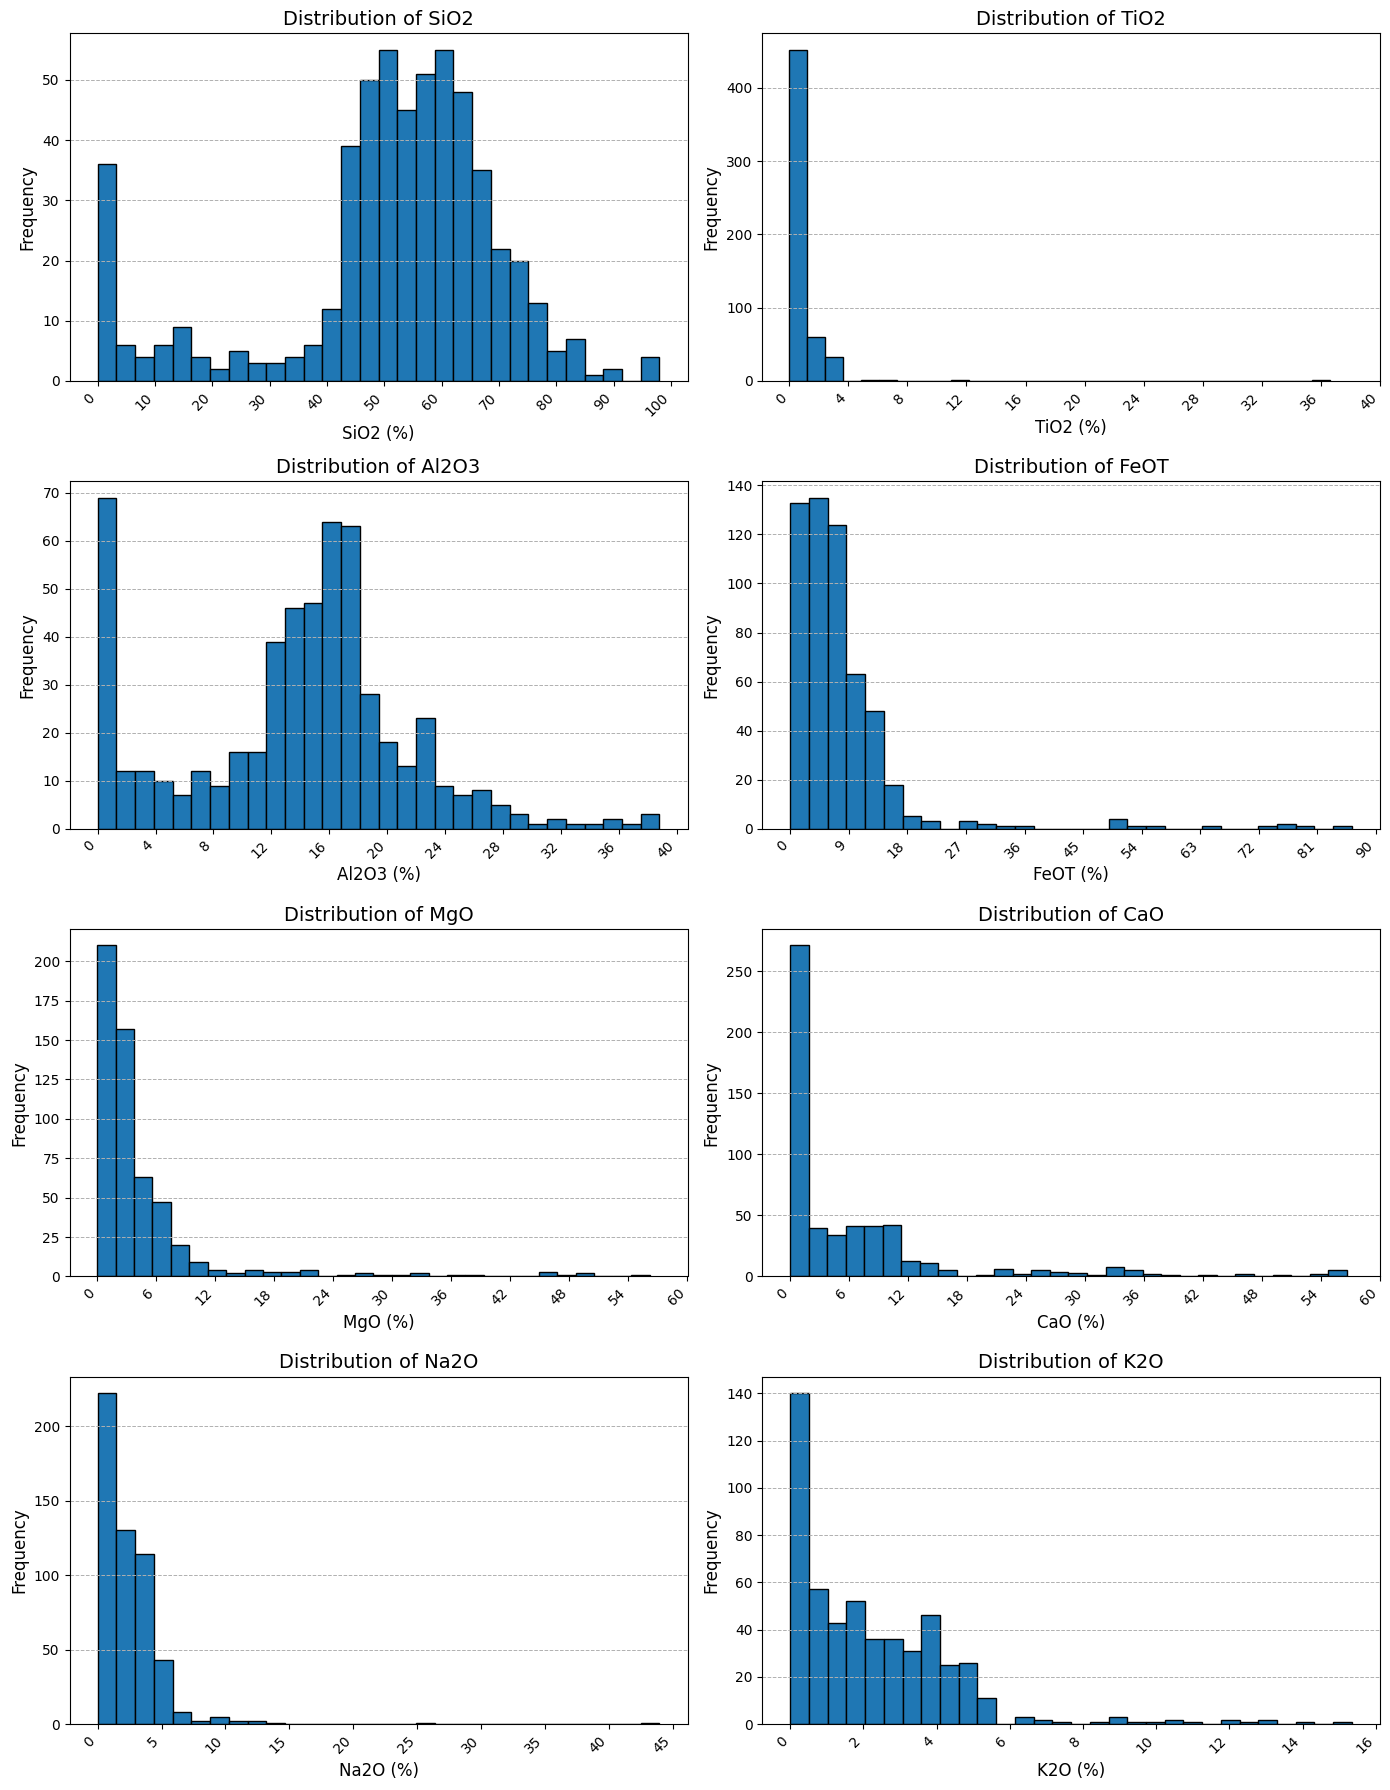
\includegraphics[width=\textwidth]{images/oxide_distributions.png}
    \caption{Distributions of various oxide concentrations in the dataset. The histograms show the frequency of concentration values for \ce{SiO2}, \ce{TiO2}, \ce{Al2O3}, \ce{FeO_T}, \ce{MgO}, \ce{CaO}, \ce{Na2O}, and \ce{K2O}.}
    \label{fig:oxide_distributions}
\end{figure*}

Figure~\ref{fig:oxide_distributions} illustrates the distributions of various oxide concentrations in our dataset.
Across all oxides, there is a general pattern of skewed distributions, with concentrations heavily weighted towards lower values.
This is particularly notable in \ce{TiO2}, \ce{FeO_T}, \ce{MgO}, \ce{CaO}, and \ce{Na2O}.
\ce{SiO2} and \ce{Al2O3} show more variability, with \ce{SiO2} exhibiting a bimodal distribution.
These distributions confirm the presence of extreme values across all oxides, which are significantly overrepresented or underrepresented, further complicating the model training process.

This necessitates careful dataset partitioning to ensure that the model training process accounts for these challenges, improving the generalizability and robustness of the models.

\subsubsection{Dataset Partitioning}\label{subsubsec:dataset_partitioning}
To ensure rigorous evaluation of our models and to address the challenges of data leakage and uneven distribution of extreme values, we have implemented a customized k-fold cross-validation procedure.
This procedure ensures that all data points from a given target are either entirely in the training set or the test set, overcoming the challenge of data leakage we mention above.
Additionally, it ensures that extreme values are handled appropriately to maintain an even distribution across folds, as demonstrated by the data distributions in Figure~\ref{fig:oxide_distributions}.

\begin{algorithm}
\caption{Data Partitioning With Extreme Value Handling}
\label{alg:custom_kfold_cv}
\begin{algorithmic}[1]
\Require Dataset \( \mathbf{D} \), group column \( g \), target column \( t \), number of splits \( k \), percentile \( p \), random seed \( \textit{seed} \)
\Ensure Cross-validation folds \( \mathbf{F}_\text{cv} \), training set \( \mathbf{D}_\text{train} \), and test set \( \mathbf{D}_\text{test} \)
\State \label{line:seed} Set random seed for reproducibility if \(\text{seed} \) is not None
\State \label{line:remove_duplicates} Remove duplicate entries based on \( g \) and sort by \( t \)
\State \label{line:assign_folds} Assign fold numbers sequentially from 0 to \( k-1 \) to unique targets
\If{extreme values handling is enabled}
    \State \label{line:identify_extremes} Identify extreme values at percentiles \( p \) and \( 1-p \)
    \State \label{line:reassign_extremes} Reassign extreme values to folds \( 0 \) to \( k-2 \)
\EndIf
\State \label{line:merge_folds} Merge fold assignments back into the original dataset
\State \label{line:split_dataset} Split dataset into test set \( \mathbf{D}_\text{test} \) (fold \( k-1 \)) and remaining data \( \mathbf{D}_\text{train} \)
\State \label{line:create_folds} Create \( k-1 \) training and validation folds
\For{each fold \( i \) from 0 to \( k-2 \)}
    \State \( \mathbf{F}_\text{train}[i] \gets \mathbf{D}_\text{train} \setminus \text{fold}_i \)
    \State \( \mathbf{F}_\text{val}[i] \gets \text{fold}_i \)
    \State Append \((\mathbf{F}_\text{train}[i], \mathbf{F}_\text{val}[i])\) to \(\mathbf{F}_\text{cv}\)
\EndFor
\State \label{line:remove_fold_column} Remove fold column from all datasets
\State \Return \( \mathbf{F}_\text{cv}, \mathbf{D}_\text{train}, \mathbf{D}_\text{test} \)
\end{algorithmic}
\end{algorithm}

The procedure outlined in Algorithm~\ref{alg:custom_kfold_cv} begins by setting a random seed for reproducibility if one is provided (Line~\ref{line:seed}).
This ensures that the results are consistent across different runs of the algorithm.
Next, the dataset is processed to remove any duplicate entries based on the group column and then sorted by the target column (Line~\ref{line:remove_duplicates}).
This step ensures that each group is uniquely identified and ordered appropriately.
The dataset we illustrate in Table~\ref{tab:final_dataset_example} would require a group column $g$ of "\texttt{Target}" to group the data by target.
The target column $t$ refers to the column with the target variable, which would be the oxide for which we are predicting the concentration, for example, \ce{SiO_2}.
By sorting the dataset by the target column, we ensure that the data is ordered by the target concentration values in ascending order.

Fold numbers are then assigned sequentially using a modulo operation to ensure a random-like distribution of the unique targets across the folds (Line~\ref{line:assign_folds}).
This means that, while the assignment process follows a sequence, the resulting distribution of targets is effectively randomized.
If handling of extreme values is enabled, the algorithm identifies the top and bottom percentiles of the target values (Line~\ref{line:identify_extremes}) and reassigns these extreme values to the training folds (0 to \( k-2 \)) to ensure they are well-represented during model training (Line~\ref{line:reassign_extremes}).

The fold assignments are then merged back into the original dataset, as described in Line~\ref{line:merge_folds}.
Following this, the dataset is divided into a test set, which always consists of the data points assigned to fold \( k-1 \), and the remaining data forms the training set, as outlined in Line~\ref{line:split_dataset}.
The training data is further divided into \( k-1 \) folds for cross-validation.
For each fold, the training data consists of all but one fold, which serves as the validation set.
These pairs of training and validation sets are then appended to the list of cross-validation folds \(\mathbf{F}_\text{cv}\) (Line~\ref{line:create_folds}).

Finally, the fold indicator column is removed from all datasets before returning the final partitions (Line~\ref{line:remove_fold_column}).
The fold indicator column was added to keep track of which data points belong to which folds, which is crucial for ensuring that data points are correctly partitioned into their respective training and test sets during cross-validation. 
This cleanup step ensures that the fold information does not interfere with subsequent data processing or model training.

The final output of this procedure consists of:
\begin{itemize}
    \item The cross-validation folds \(\mathbf{F}_\text{cv}\), each containing a tuple of training and validation sets.
    \item The training set \(\mathbf{D}_\text{train}\) in its entirety.
    \item The test set \(\mathbf{D}_\text{test}\), distinct from the training set.
\end{itemize}

The data partitioning does not modify the original dataset, it merely partitions it.
For that reason, each of the datasets that are returned have the same structure as shown in Table~\ref{tab:final_dataset_example}.

By following this procedure, we ensure that our cross-validation is robust against data leakage, maintains the integrity of grouped targets, and carefully handles extreme values to improve the representativeness of the training set.

Our method is inspired by the approach described by \citet{andersonImprovedAccuracyQuantitative2017}.
They employed a similar strategy to assess the performance of their PLS model, using k-fold cross-validation and a separate test set.
Their process involved dividing the full set of laboratory data into five folds, using four for cross-validation and combining them as the final training set, while the fifth fold served as a test set.
This approach ensured that each fold represented the full elemental compositional variation, and extreme targets were included in the training folds to handle a wider range of compositions.
For consistency, we also use \(k=5\) for our cross-validation.

Additionally, by using $k=5$ folds, we have effectively chosen an 80\%/20\% split between the training and testing datasets.
In our experience, this ratio maximizes the training set's capacity for effective model learning while ensuring that the testing set is sufficiently representative to provide an accurate assessment of the model's performance on new data.
Allocating too much data to the testing set could compromise the comprehensiveness of the training set, undermining the model's ability to generalize effectively due to the limited availability of data.
